%%%%%%%%%%%%%%%%%%%%%%%%%%%%%%%%%%%%%%%%%
% baposter Landscape Poster
% LaTeX Template
% Version 1.0 (11/06/13)
%
% baposter Class Created by:
% Brian Amberg (baposter@brian-amberg.de)
%
% This template has been downloaded from:
% http://www.LaTeXTemplates.com
%
% License:
% CC BY-NC-SA 3.0 (http://creativecommons.org/licenses/by-nc-sa/3.0/)
%
%%%%%%%%%%%%%%%%%%%%%%%%%%%%%%%%%%%%%%%%%

%----------------------------------------------------------------------------------------
%	PACKAGES AND OTHER DOCUMENT CONFIGURATIONS
%----------------------------------------------------------------------------------------

\documentclass[portrait,a0paper,fontscale=0.285, margin=30mm]{baposter} % Adjust the font scale/size here

\usepackage{graphicx} % Required for including images
\graphicspath{{figures/}} % Directory in which figures are stored

\usepackage{amsmath} % For typesetting math
\usepackage{amssymb} % Adds new symbols to be used in math mode

\usepackage{subfig}

\usepackage{bm}

\usepackage{graphicx}
\usepackage{graphics}
 \usepackage[parfill]{parskip}				
 \usepackage{pstricks}
\usepackage{subfig}
\usepackage{enumerate}
\usepackage{xspace}
\usepackage{cite}
\usepackage{anyfontsize}
\usepackage{booktabs} % Top and bottom rules for tables
\usepackage{enumitem} % Used to reduce itemize/enumerate spacing
\usepackage{palatino} % Use the Palatino font
\usepackage[font=small,labelfont=bf]{caption} % Required for specifying captions to tables and figures
 \usepackage{vwcol}  


\usepackage{multicol} % Required for multiple columns
\setlength{\columnsep}{1.5em} % Slightly increase the space between columns
\setlength{\columnseprule}{0mm} % No horizontal rule between columns

\usepackage{tikz} % Required for flow chart
\usetikzlibrary{shapes,arrows} % Tikz libraries required for the flow chart in the template

\newcommand{\compresslist}{ % Define a command to reduce spacing within itemize/enumerate environments, this is used right after \begin{itemize} or \begin{enumerate}
\setlength{\itemsep}{1pt}
\setlength{\parskip}{0pt}
\setlength{\parsep}{0pt}
}

\definecolor{lightblue}{rgb}{0.145,0.6666,1} % Defines the color used for content box headers

\begin{document}

\begin{poster}
{
headerborder=closed, % Adds a border around the header of content boxes
colspacing=1em, % Column spacing
bgColorOne=white, % Background color for the gradient on the left side of the poster
bgColorTwo=white, % Background color for the gradient on the right side of the poster
borderColor=lightblue, % Border color
headerColorOne=black, % Background color for the header in the content boxes (left side)
headerColorTwo=blue, % Background color for the header in the content boxes (right side)
headerFontColor=white, % Text color for the header text in the content boxes
boxColorOne=white, % Background color of the content boxes
textborder=roundedleft, % Format of the border around content boxes, can be: none, bars, coils, triangles, rectangle, rounded, roundedsmall, roundedright or faded
eyecatcher=true, % Set to false for ignoring the left logo in the title and move the title left
headerheight=0.10\textheight, % Height of the header
headershape=roundedright, % Specify the rounded corner in the content box headers, can be: rectangle, small-rounded, roundedright, roundedleft or rounded
headerfont=\Large\bf\textsc, % Large, bold and sans serif font in the headers of content boxes
%textfont={\setlength{\parindent}{1.5em}}, % Uncomment for paragraph indentation
linewidth=2pt, % Width of the border lines around content boxes
columns=5
}
%----------------------------------------------------------------------------------------
%	TITLE SECTION 
%----------------------------------------------------------------------------------------
%
{
\includegraphics[width=0.14\textwidth]{figures hugo/logoIGE.png}} % First university/lab logo on the left
{{\fontsize{16}{40}\selectfont\bf\textsc{Atmospheric boundary layer response \\ to oceanic sub-mesoscale SST fronts}}  } % Poster title
{\Centering\textsc{\fontsize{13}{40}\selectfont\textsc{Hugo Jacquet$^{1}$, Alex Ayet$^2$ and Fleur Couvreux$^3$}   \vspace{0.3em}\newline 
 {\fontsize{9.}{40}\selectfont$^1$ IGE, CNRS, Grenoble}
  {\fontsize{9.}{40}\selectfont$^2$ GIPSA, CNRS, Grenoble}
   {\fontsize{9.}{40}\selectfont$^3$ CNRM, Météo-France, Toulouse}}}
% Author names and institution
{
\includegraphics[width=0.15\textwidth]{figures hugo/logoCNRS.png}} % Second university/lab logo on the right

%----------------------------------------------------------------------------------------
%	OBJECTIVES
%----------------------------------------------------------------------------------------
\vspace{0.3em}
\headerbox{Motivation}{name=introduction,column=0,row=0, span=2}{
{\fontsize{10}{40}\selectfont
Surface heterogeneities can greatly affect the atmospheric boundary layer (ABL), through changes in surface roughness, humidity, or heat fluxes. Recent improvements of satellite imagery allow observing the response of the ABL to such heterogeneities at small scales (see the “Case Study” pannel). Those images suggest that the ABL response could be scale-dependent  (e.g. advection could play a non negligible role). While this type of air-sea interactions has been largely studied at larger scales [1], atmosphere response to SST front of width of 1-10km is not well understood [2][3].\\
The goal of this study is to provide an understanding of the processes at stake in the atmosphere response to sub-mesoscale sea surface temperature (SST) fronts.}}

%----------------------------------------------------------------------------------------
%	CLOUD INDEX
%----------------------------------------------------------------------------------------
\headerbox{LES overview}{name=cloud,column=3,row=1, span=2,  below=introduction}{

\includegraphics[width=\textwidth]{figures hugo/LSwind_and_UVprofiles_v2.png}
%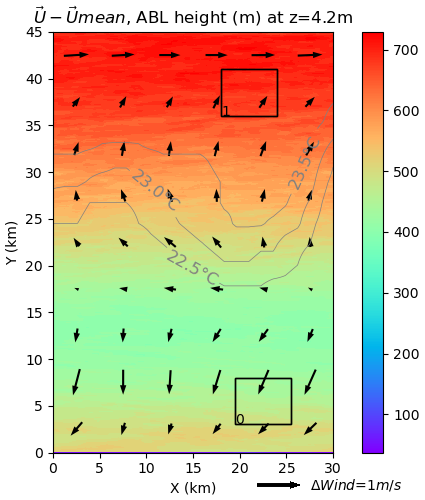
\includegraphics[width=0.53\textwidth]{figures hugo/largescale_wind_z2_s50.png} 
%\vspace{0.3em}
%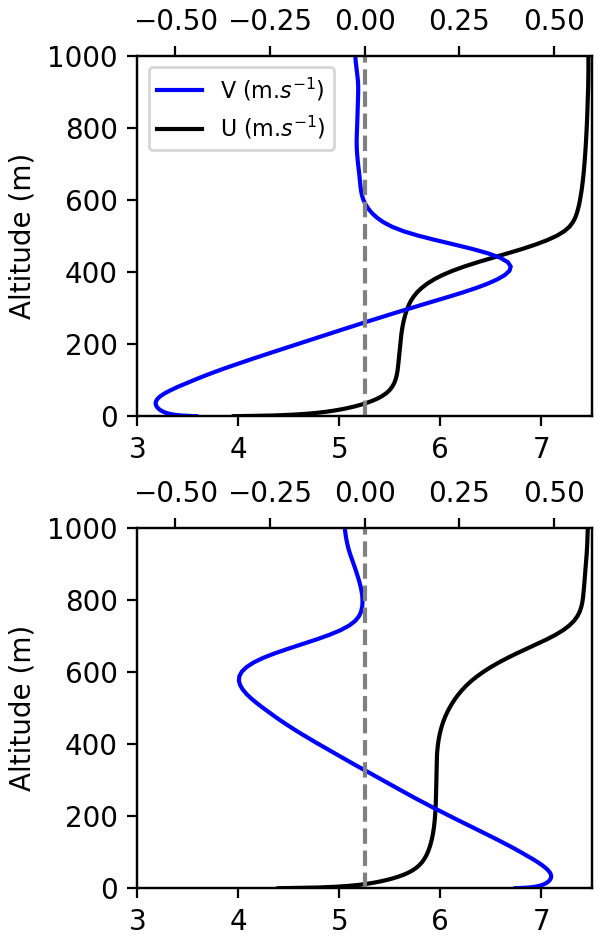
\includegraphics[width=0.46\textwidth]{figures hugo/profiles_UV.png} 
%\includegraphics[height=80pt]{figures/clear_sky.png}
%\begin{multicols}{2}
\begin{itemize}[label=\textbullet, font=\small]
    \item LES on a 30km x 45km x 2000m domain, $\Delta$x=$\Delta$y=50 m $\Delta$z in [2,20] m,(86.4x$10^6$ grid cells)
    
    \item Boundaries: N/S open, E/W cyclic.
        initial wind (U,V) = (7.5,0) $m.s^{-1}$, N$^{2}$ = 10$^{-4}$ $s^{-2}$
    \item MesoNH model, 20h run. No moisture, clouds or radiation. Date = 10/12/2015
\end{itemize}
%\end{multicols}
%\vspace{1pt}
}
\headerbox{Case study: Agulhas current}{name=mask ,column=2,row=0,  span=3}{


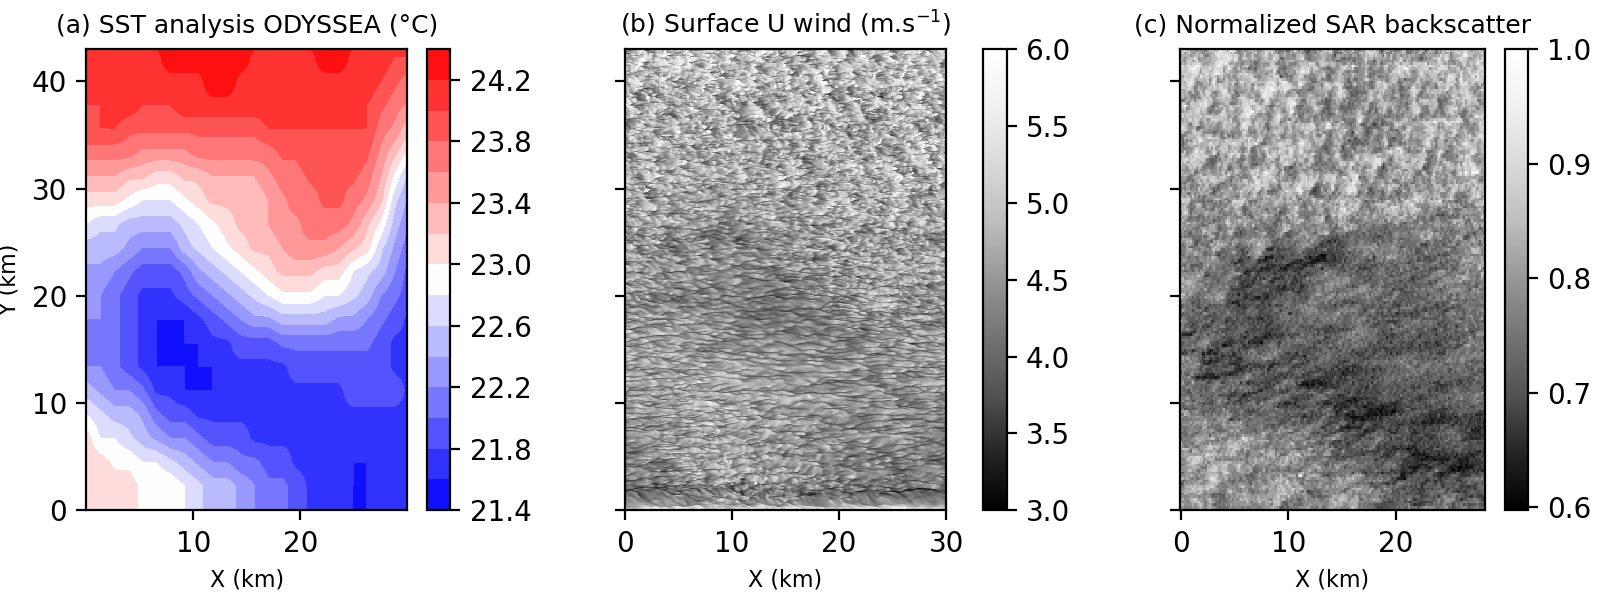
\includegraphics[width=\textwidth]{figures hugo/SST_Usurface_SAR.png}
The simulation is in the Agulhas current region, over a strong SST gradient (2° over 10km). The mean wind is mostly along the x direction, as is the general direction of iso-SST. This is referred as a 'along-front' configuration.
}

%----------------------------------------------------------------------------------------
%	Features
%----------------------------------------------------------------------------------------
\headerbox{Processes}{name=id, column=0,span=3,row=1, below=mask}{

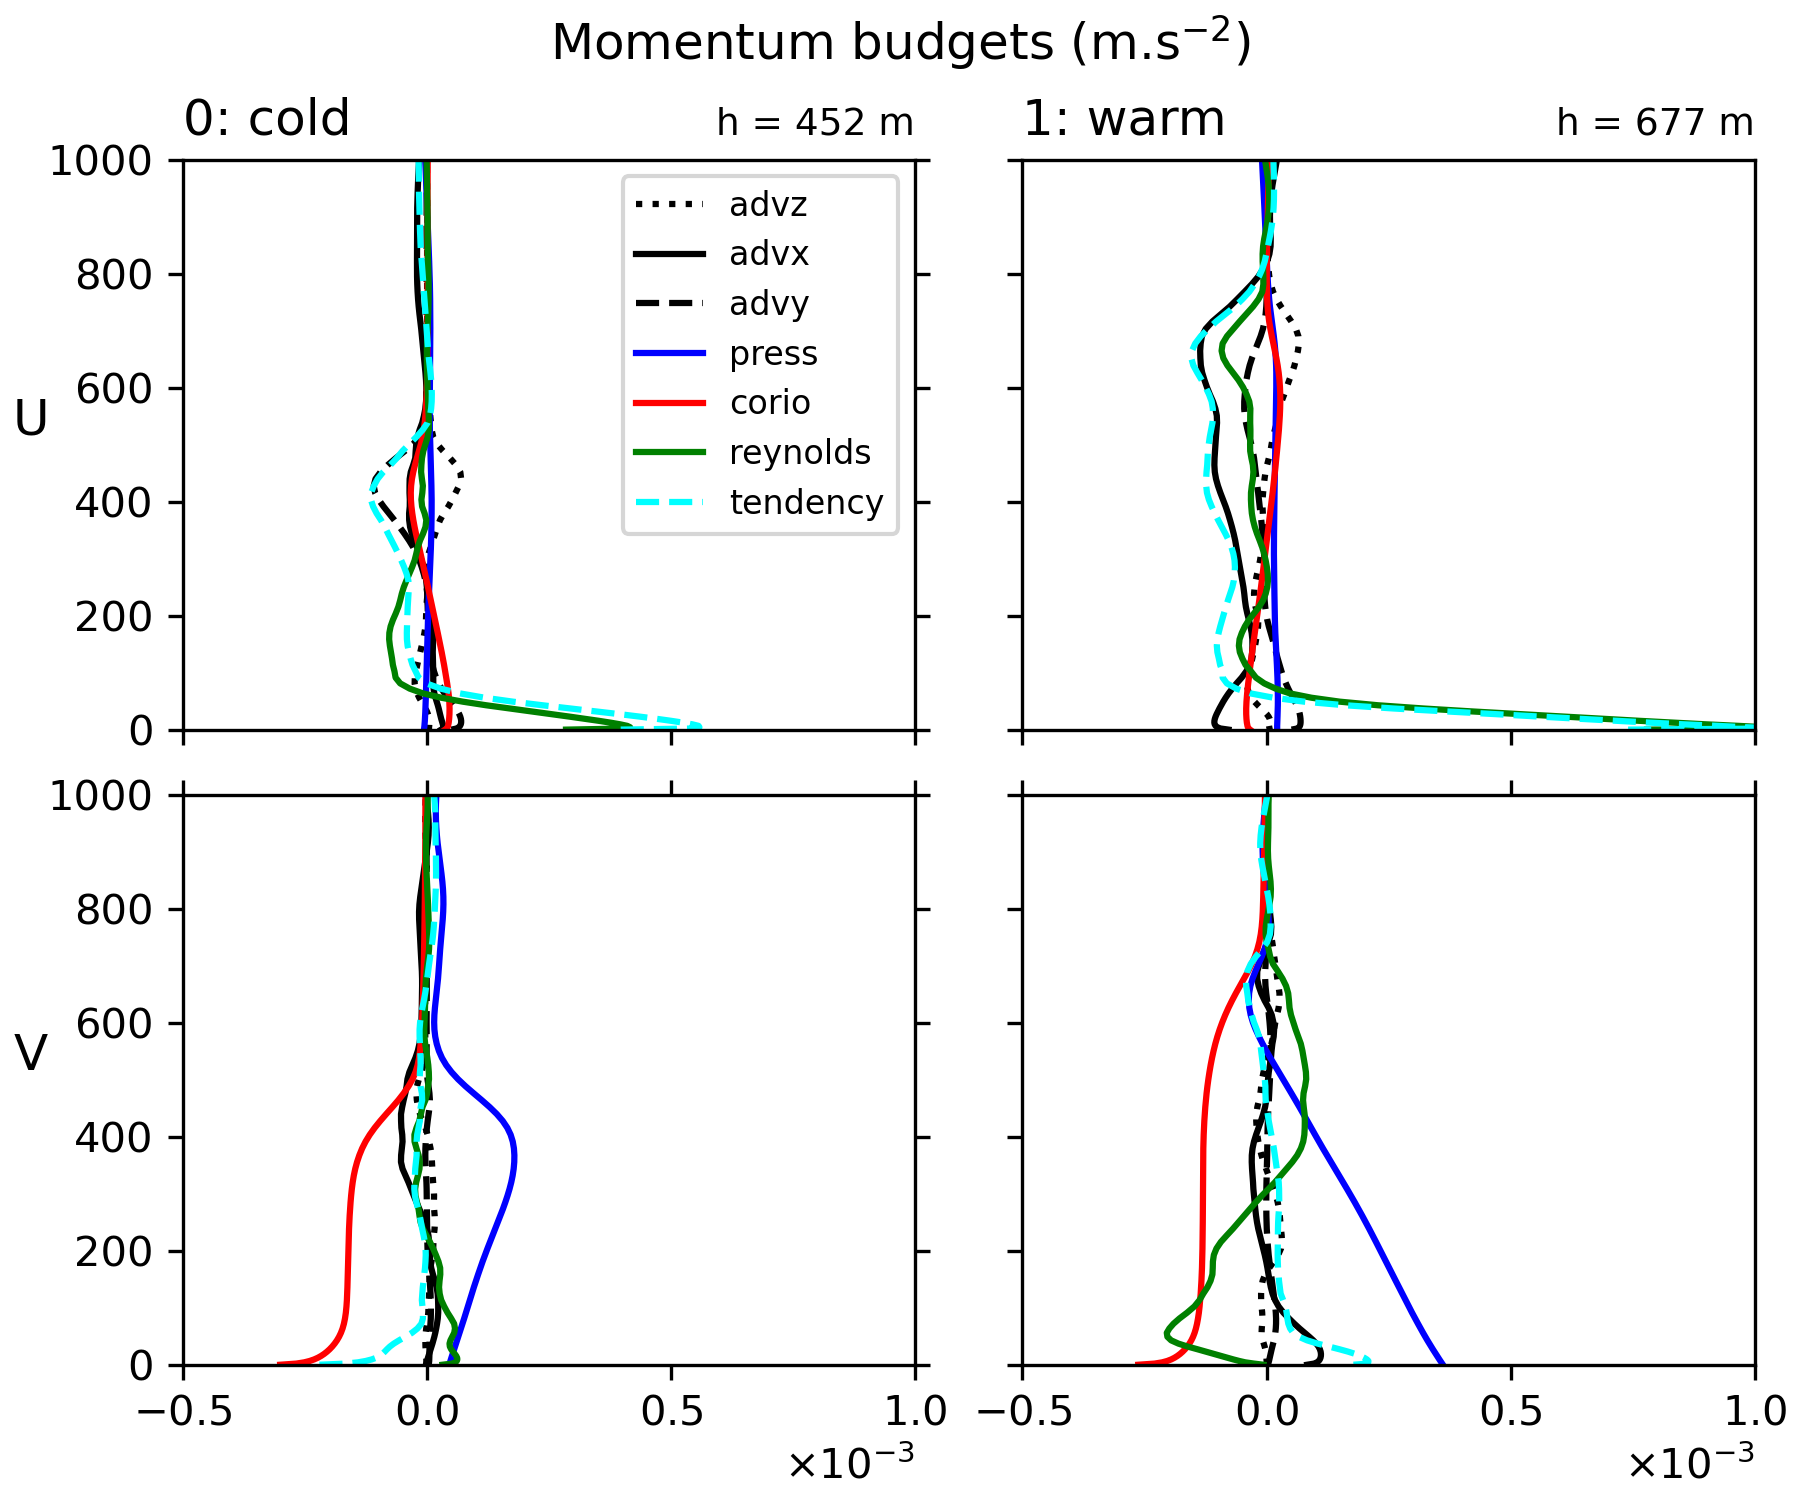
\includegraphics[width=\textwidth]{figures hugo/UV_budget_temporalmean_V2.png}
\includegraphics[width=\textwidth]{figures hugo/UVWthtv_X400_modified.png}

\begin{multicols}{2}
\textbullet \hspace{0.2cm} On warm SST, the turbulent (buoyant) production is enhanced: faster wind from aloft is mixed towards the surface, accelerating the surface winds and slowing upper layers.

\textbullet \hspace{0.2cm} Two V secondary circulations have formed ('LES overview' panel, right), with well marked upward motion but more diffuse subsidence, maintained by a north/south pressure gradient and Coriolis forces. 

\textbullet \hspace{0.2cm} The ABL height is increased from cold to warm SST, suggesting that SST heterogeneities can modify the whole ABL. Surface large scale winds show a divergence aligned with the mean wind but no fully bi-dimension heterogeneity ('LES overview' panel, left). 
\end{multicols}
}
%The ABL height is computed as the height at which the potential temperature is equal to the integrated potential temperature of lower heights plus 0,25K.
%----------------------------------------------------------------------------------------
%	CONCLUSION
%----------------------------------------------------------------------------------------

\headerbox{Conclusion}{name=aggr,column=3,row=2,span=2, below=cloud }{
Winds are directly modified by the bidimensional SST heterogeneity, while bulk properties such as the boundary layer height is only influenced by a global north/south SST gradient. \\

Other simulations will be conducted, with 1D SST front in a canal geometry.
Taking into account moist and clouds could change the dynamics of the processes and should be investigated. 
}
\headerbox{References}{name=aggr,column=3,row=3,span=2, below=aggr }{{\fontsize{7}{40}\selectfont
[1] Kilpatrick, T., N. Schneider, and B. Qiu, 2016: Atmospheric Response to a Midlatitude SST Front: Alongfront Winds. J. Atmos. Sci., 73, 3489–3509, https://doi.org/10.1175/JAS-D-15-0312.1. \newline
[2] Wenegrat, J. O., \& Arthur, R. S. (2018). Response of the atmospheric boundary layer to submesoscale sea surface temperature fronts. Geophysical Research Letters, 45, 13,505– 13,512. https://doi.org/10.1029/2018GL081034 \newline
[3] Sullivan, P. P., J. C. McWilliams, J. C. Weil, E. G. Patton, and H. J. S. Fernando, 2021: Marine Boundary Layers above Heterogeneous SST: Alongfront Winds. J. Atmos. Sci., 78, 3297–3315, https://doi.org/10.1175/JAS-D-21-0072.1. }
}

\end{poster}

\end{document}\grid
\grid
